\section{Ordinary Differential Equations (ODEs)}

% AIMS: cut as with other sections.
%\subsection*{Aims}
%\begin{itemize}
%\item Describing basic ideas of ODEs
%\item Solve first order ODEs
%\item Solve linear second order ODEs
%\end{itemize}

Differential equations are widely used in science, engineering and economics.  After 400 years there are still lots of open problems to solve.

\subsection{Overview}

A differential equation is an equation which links $y$,\quad
$\dfrac{dy}{dx}$, \quad $\dfrac{d^2 y}{dx^2}$, etc.

\begin{examples}\quad
\begin{tabular}{ll}
$\dfrac{dy}{dx}  =  x$ & Easy \\
$\dfrac{dy}{dx}  =  x + y^2$ & Hard \\
$\left(\dfrac{dy}{dx}\right)^2 + \left(\dfrac{dy}{dx}\right)  =  \sin(y)$ & Very hard \\
$\dfrac{d^2y}{dx^2} + \dfrac{dy}{dx}  =  \sin(x)$ & Easy
\end{tabular}
\end{examples}

``Ordinary'' means there is only one independent variable.

\subsection*{Some terminology}

\begin{itemize}
\item The \textbf{order} of a differential equation is the largest
number of derivatives.

\begingroup
\renewcommand{\arraystretch}{2}
\begin{tabular}[3]{ll}
$\dfrac{dy}{dx}  =  x$ & \textbf{First} order \\
$\dfrac{d^2y}{dx^2}  =  x$ & \textbf{Second} order \\
$\dfrac{d^4y}{dx^4} + p \dfrac{d^2y}{dx^2} + y  =  0$ &
\textbf{Fourth} order
\end{tabular}
\endgroup

\item A differential equation is \textbf{linear} if we only have
$\dfrac{d^2y}{dx^2}$, $\dfrac{dy}{dx}$ or $y$ and no functions such
as $y^2$.

\begin{itemize}
\item Linear equations are easy to solve and very common.

\item Nonlinear equations are often \textbf{very} hard to
solve.  The solutions usually use numerical methods.
\end{itemize}

\item The \textbf{initial condition(s)} of a differential equation
is information about the solution at a point $x=a$. We need this to find a particular solution to the equation; that is, one that does not depend on any arbitrary constants.

\begin{tabular}{ll}
 First order: & Need to know $y(a)$ \\\\
 Second order: & Need to know $y(a)$, $\dfrac{dy(a)}{dx}$
\end{tabular}
\end{itemize}



\subsection{Separable first order differential equations}  \label{sect:sepdiff}

\begin{definition}
A \textbf{separable} first order ordinary differential equation has
the form
\[
\dfrac{dy}{dx}  =  p(x)q(y).
\]
\end{definition}

We can solve these \textbf{directly by integration}:

Rearrange and integrate
\begin{align*}
\dfrac{1}{q(y)} \dfrac{dy}{dx}  & =  p(x)  \\
\implies \int \dfrac{1}{q(y)} \dfrac{dy}{dx}dx & = \int p(x)dx  \\
\implies \int \dfrac{dy}{q(y)} & =  \int p(x)dx
% \label{sepde_eqn}
\end{align*}

\begin{example}
 \[
  \dfrac{dy}{dx} = \dfrac{xe^{x^2}}{y^2}
 \]

 Separate and integrate
 \begin{eqnarray*}
  && \int y^2 dy = \int x e^{x^2} dx\\
  &\Rightarrow& \dfrac{y^3}{3} = \dfrac{1}{2} e^{x^2} + c\\
  &\Rightarrow& {y^3} = \dfrac{3}{2} e^{x^2} + c 
 \end{eqnarray*}

\end{example}

\begin{example}
In the introduction to the course we saw a basic model for world population.  A more sophisticated model for population $p(t)$ might satisfy the differential equation
\[
\dfrac{dp}{dt}  = p(M-p).
\]

Separating variables and integrating gives
\begin{eqnarray*}
&& \int \dfrac{dp}{p(M-p)}  =  \int dt \\
& &\text{LHS use partial fractions} \\
&& \dfrac{1}{p(M-p)}  =  \dfrac{\dfrac{1}{M}}{p} +
\dfrac{\dfrac{1}{M}}{M-p} \\
&\therefore & \dfrac{1}{M} \ln \left|\dfrac{p}{M-p}\right|
 =  t + C.
\end{eqnarray*}

To find $C$ we need some initial data. Let $p=p_0$ at $t=0$.
\begin{eqnarray*}
&\Rightarrow  & C  =  \dfrac{1}{M} \ln \left|\dfrac{p_0}{M-p_0}\right| \\
&\therefore & \dfrac{1}{M} \ln \left|\dfrac{p}{M-p}\right|
 =  t + \dfrac{1}{M} \ln \left|\dfrac{p_0}{M-p_0}\right|.
\end{eqnarray*}

Multiply by $M$ and exponentiate
\[
\frac{p}{M-p}  =  \dfrac{p_0}{M-p_0} e^{Mt}.
\]

Rearrange
\begin{eqnarray*}
&& p  =  \left[ \dfrac{p_0}{M-p_0} e^{Mt}\right] M - \left[
\dfrac{p_0}{M-p_0} e^{Mt}\right]p \\
&& p\left[1 + \dfrac{p_0}{M-p_0} e^{Mt}\right] = \left( \dfrac{p_0
M}{M-p_0}\right) e^{Mt}
\end{eqnarray*}
\begin{eqnarray*}
\therefore \quad  p  &=&  \dfrac{M p_0 e^{Mt}}{M-p_0+p_0 e^{Mt}}\\
&=&  \dfrac{M p_0 e^{Mt}}{M-p_0} \cdot  \dfrac{M - p_0}{M-p_0+p_0 e^{Mt}}
\end{eqnarray*}
% The last expression doesn't seem helpful.

Sketch:

At $t=0$, 
\[
p = \dfrac{M p_0}{M - p_0 + p_0}=p_0.
\]

As $t \to \infty$,
\[
 \dfrac{Mp_0}{p_0} = M.
\]

%% \nextalt{Request description from lecturer or tactile diagram.}
\begin{figure}[H]
\centering
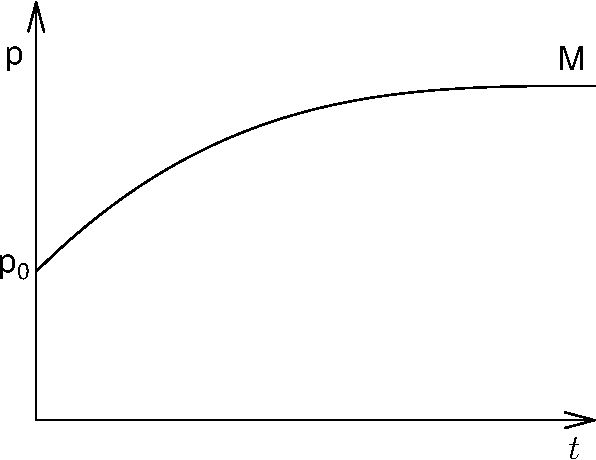
\includegraphics[width=0.5\textwidth]{population-de.pdf}
\caption{Sketch of example}
\label{populationde}
\end{figure}

\end{example}



\subsection{Homogeneous equations}

A function $f(x,y)$ is homogeneous of degree $n$ if
\[
 f(tx,ty) = t^{n} f(x,y).
\]

\begin{examples}
 \quad
 \begin{eqnarray*}
   f(x,y) &=& x^2 + xy\\
  \Rightarrow\quad f(tx, ty) &=& t^2 x^2 + t^2 xy \\
  &=& t^2 f(x,y)
 \end{eqnarray*}
(homogeneous, degree $2$)

 \begin{eqnarray*}
   f(x,y) &=& \sqrt{x^2 + y^2}\\
  \Rightarrow\quad f(tx, ty) &=& t \sqrt{x^2 + y^2} \\
  &=& t f(x,y)
 \end{eqnarray*}
(homogeneous, degree $1$)

\[
 f(x,y) = \sin \left(\dfrac{y}{x}\right)
\]
(homogeneous, degree $0$)
\end{examples}


% There's no higher degree version, but it looks like it is possible to use a similar method using t = 1/x.
\subsubsection*{Degree $0$.}

The general form for a homogeneous differential equation of degree $0$ is
\[
 \dfrac{dy}{dx} = f \left(\dfrac{y}{x}\right)
\]

\begin{solution}
 Let $u=\dfrac{y}{x}$. Then
 \begin{eqnarray*}
  && ux = y\\
  &\Rightarrow& u+x \dfrac{du}{dx} = \dfrac{dy}{dx}.
 \end{eqnarray*}

 Hence
  \begin{eqnarray*}
  && u + x \dfrac{du}{dx} = f(u)\\
  &\Rightarrow& x \dfrac{du}{dx} = f(u) - u\\
  &\Rightarrow& \int \dfrac{du}{f(u)-u} = \int \dfrac{dx}{x} = \ln \left|x\right|+c.
 \end{eqnarray*}
\end{solution}

\begin{example}
 \[
  \dfrac{dy}{dx} = \dfrac{y}{x} \left(1 + \ln \left(\dfrac{y}{x}\right)\right)
 \]
 
 Let $u=\dfrac{y}{x}$. Then
 \begin{eqnarray*}
  u + x \dfrac{du}{dx} &=& u (1 + \ln(u))\\
  &=& u + u \ln (u)\\
  \Rightarrow \quad \int \dfrac{du}{u \ln(u)} &=& \int \dfrac{dx}{x} \\
  &=& \ln \left|x\right| + c.
 \end{eqnarray*}

 Let $v=\ln(u)$. Then
 \[
  \dfrac{dv}{du} = \dfrac{1}{u} \qquad (u>0)
 \]

 So
 \[
  \int \dfrac{du}{u \ln(u)} = \int \dfrac{dv}{v} = \ln \left|v\right|
 \]
 
 Hence
 \[
  \ln \left|v\right| = \ln (x)+c
 \]
 
 If $v>0$, \quad $v=Ax$, \quad $A=e^{c}$.

\begin{eqnarray*}
& \Rightarrow & \ln (u) = Ax\\
& \Rightarrow & \ln \left(\dfrac{y}{x}\right) = Ax\\
& \Rightarrow & u=xe^{Ax}.
\end{eqnarray*}
\end{example}


\subsection{Linear first order ordinary differential equations}

These take the form
\begin{equation*}
\dfrac{dy}{dx} + p(x)y  =  q(x).
\label{lin_ODE}
\end{equation*}
The LHS is a linear combination of $y$ and its derivative.


We solve these by using an \textbf{integrating factor}. 


\begin{lemma}
If $r(x) = e^{\int p(x)dx}$ then
\[
\dfrac{dr}{dx}  =  p(x) r(x).
\]
\end{lemma}

\begin{Proof}
By chain rule
\begin{eqnarray*}
 \dfrac{dr}{dx}  &=&  e^{\int p(x)dx} \dfrac{d}{dx} \int
p(x)dx\\
&=& p(x) e^{\int p(x)dx} \\
&& \text{by Fundamental theorem of calculus}\\
&=& p(x) r(x)
\end{eqnarray*}
\end{Proof}

The function $r(x) =  e^{\int p(x)dx}$ is called the \emph{integrating factor}.

\begin{proposition}
The equation
\begin{equation}
 \dfrac{dy}{dx} + p(x)y = q(x)
 \label{eq5.1}
\end{equation}
has solution
\[
 y(x) = \dfrac{1}{r(x)} \int r(x)q(x)dx.
\]
\end{proposition}

\begin{Proof}
Consider
\begin{eqnarray*}
 && \dfrac{d}{dx} (r(x)y(x)) \\
 &=& r(x) \dfrac{dy}{dx} + y \dfrac{dr}{dx}\\
 &=& r(x) \dfrac{dy}{dx} + y pr\\
 &=& r(x) \left(\dfrac{dy}{dx} + y p\right)
\end{eqnarray*}

Hence if $y$ satisfies \eqref{eq5.1}, then
\begin{eqnarray*}
 && \dfrac{d}{dx}(ry) = r \left(\dfrac{dy}{dx}+py\right) = rq\\
 &\Rightarrow& y = \dfrac{1}{r} \int rq dx.
\end{eqnarray*}
\end{Proof}


\begin{examples}
\quad

\begin{enumerate}
 \item $\dfrac{dy}{dx} + y  =  x$

 So
 \[
  \dfrac{dy}{dx} + p(x)y = q(x),
 \]
where
\[
p(x) = 1, \quad q(x) = x.
\]

Integrating factor:
\begin{eqnarray*}
r(x) = e^{\int p(x)dx}
 =  e^x.
 \end{eqnarray*}
 
Hence
\begin{eqnarray*}
y(x) &=&  e^{-x} \int e^x x dx\\
&=&  e^{-x} [xe^{x} - e^{x} + c]\\
&=&  x - 1 + ce^{-x}.
\end{eqnarray*}
(note: non-trivial constant)

\item $x \dfrac{dy}{dx} + 2 u  =  x^3$

Rearranging,
\[
 \frac{dy}{dx} + 2 \frac{y}{x}  =  x^2 ,
\]
so
\[
 \frac{dy}{dx} + p(x)y  =  q{x}, 
\]
where $p(x)=\dfrac{2}{x}$, $q(x) = x^2$.

Integrating factor:
\begin{eqnarray*}
 r(x) &=& e^{\int \frac{2}{x}dx} \\
 &=& e^{2\ln(x)}\\
 &=& x^2.
\end{eqnarray*}

Hence
\begin{eqnarray*}
 y(x) &=& \dfrac{1}{x^2} \int x^2 x^2 dx \\
 &=& \dfrac{1}{x^2} \left[\dfrac{x^5}{5}+c\right]\\
 &=& \dfrac{x^3}{5} + \dfrac{c}{x^2}.
\end{eqnarray*}

% I have never done this long and tedious example in the lecture.
% Omitting it from the lecture notes for now.

%% Definitely a problems class example.
%% Also from "Now, for constants..." I think it could use some work to make it more easy to follow.
%\item Climate: Why is February such a rotten month (in England)?
%
%\nextalt{Request description from lecturer or tactile diagram.}
%\begin{figure}[H]
%\centering
%\includegraphics[width=0.55\textwidth]{climate.pdf}
%\caption{Climate}
%\label{climate}
%\end{figure}
%
%$t$:\quad years;  $t=0$  on 21st Dec. (Winter Solstice)
%% Winter Solstice is actually 22nd December this year.
%
%$S$:\quad sunshine, modelled as
%\[
%S(t)=\overline{s} (1-\cos(2\pi t)).
%\]
%
%$T$:\quad Kelvin; the sea (surface) temperature.
%
%Newton's law of cooling:
%\[
 %\frac{dT}{dt}  =  -k (T - S(t)) 
%\]
%($k$ constant)
%
%Rearranging
%\[
 %\frac{dT}{dt} + k T  =  k S(t)
%\]
%
%So this is in the form \eqref{eq5.1}
%with $p(t)=k$, $q(t)=k S(t)$.
%
 %Integrating factor:
 %\[
  %r(t) = e^{\int kdt} = e^{kt}.
 %\]
%
 %Hence
 %\begin{eqnarray*}
  %T(t) &=& e^{-kt} \int e^{kt} k S(t) dt\\
   %&=& \overline{s} k e^{-kt} \int e^{kt} (1-\cos(2\pi t)) dt
 %\end{eqnarray*}
%
%Now, for constants $a,b\in\RR$ we have
%\begin{eqnarray*}
 %&& \int e^{at} \cos(bt) dt 
%=%\\ &=&
 %\dfrac{e^{at}}{a^2+b^2}  [a \cos(bt) + b \sin (bt)] + c.
%\end{eqnarray*}
%
%Hence the sea surface temperature is 
%\begin{eqnarray*}
%T(t) &=& \overline{s} ke^{-k t} \left(\frac{e^{k t}}{k} 
%- \frac{ e^{k t}}{k^2+4\pi^2} \left[k \cos(2\pi t) + 2\pi
%\sin(2\pi t)\right] + c\right)
%\\
%&=& \underbrace{\overline{s}}
%- \underbrace{\dfrac{\overline{s}k}{k^2+4\pi^2}
%\left[k \cos(2\pi t) + 2\pi\sin(2\pi t)\right]}
%+ \underbrace{c \overline{s} k e^{-k t}.}
%\\&&\text{base\hspace{2.5cm}seasonality\hspace{2cm}transient effect}
%\end{eqnarray*}
%
%Aside:
%\let\thhh=\theta\def\theta{\chi}%%% fix theta to chi temporarily
%
%Consider $$a \cos(x) + b \sin(x).$$
%%
%For $\theta$ such that $\tan (\theta)=\dfrac{b}{a}$ we have
%\[
 %\sin (\theta) = \dfrac{b}{\sqrt{a^2+b^2}}, \qquad \cos(\theta) = \dfrac{a}{\sqrt{a^2+b^2}}
%\]
%Then
%\begin{eqnarray*}
%&& \sqrt{a^2+b^2} \cos (x-\theta)\\
%&&= \sqrt{a^2+b^2} [\cos(x) \cos{\theta} + \sin(x) \sin(\theta)]\\
%&&= a \cos(x) + b \sin(x)
%\end{eqnarray*}
%Hence%, take $a=k,\ b=2\pi,\ x=2\pi t$,
%\begin{eqnarray*}
 %&& k \cos(2\pi t) + 2 \pi \sin(2\pi t)
 %\\ &&= 
%\sqrt{k^2+4\pi^2} \cos(2\pi t-\theta)
%\end{eqnarray*}
%where \[\tan(\theta)=\dfrac{2\pi}{k}\]
%and $\theta$ is the phase shift or lag wrt.\ the sunshine intensity $S(t)$.
%
%Thus, after transient worn off
%\[
 %T(t) \simeq \overline{s} \left(
 %1 - \dfrac{k}{\sqrt{k^2+4\pi^2}} \cos \left(2\pi\left(t-\dfrac{\theta}{2\pi}\right)\right)
 %\right)
%\]
%\\
%On our %island
%sea coast 
%$k\approx8$ is 'large', 
%%$k\approx7$, 
%%
%so $$\dfrac{\theta}{2\pi}=\dfrac{1}{2\pi}\arctan\left(\dfrac{2\pi}{k}\right)
%\approx\dfrac1k
%\approx\dfrac18\text{  (years) $\cong$ 1.5 (months),}$$
 %so the sea is coldest in February (= 21st Dec.+1.5 months).
%%\approx\dfrac19\text{  (years) $\cong$ 6 (weeks),}$$
%% so the sea is coldest in February (= 21st Dec.+6 weeks).
%
%\nextalt{Request description from lecturer or tactile diagram.}
%\iftoggle{clearprint}{
%\begin{figure}[H]
%\centering
%\boldmath
%\includegraphics[width=0.6\textwidth]{periodic_response.pdf} \\
%\raisebox{1.1cm}[0pt][0pt]{\hspace{.1cm}$/2\pi$\hspace{2.3cm}$/2\pi$}\\[-.5cm]
%\caption{Steady periodic response. Legend: $S$ -- red; $T$ -- blue.}
%\label{periodicresponse}
%\end{figure}
%}{
%\iftoggle{web}{
%\begin{figure}[H]
%\centering
%\includegraphics[width=0.6\textwidth]{periodic_response-byhand.svg}
%\caption{Steady periodic response. Legend: $S$ -- red; $T$ -- blue.}
%\label{periodicresponse}
%\end{figure}
%}{
%\begin{figure}[H]
%\centering
%\boldmath
%\includegraphics[width=0.6\textwidth]{periodic_response.pdf} \\
%\raisebox{.9cm}[0pt][0pt]{\hspace{.1cm}$/2\pi$\hspace{2.3cm}$/2\pi$}\\[-.5cm]
%\caption{Steady periodic response. Legend: $S$ -- red; $T$ -- blue.}
%\label{periodicresponse}
%\end{figure}
%}}
%\let\theta=\thhh

\end{enumerate}
\end{examples}

\subsection{Bernoulli equations}

A differential equation of the form
\[
 \dfrac{dy}{dx} + p(x)y = q(x)y^{n}, \quad n \in \ZZ
\]
is called a Bernoulli equation (named after Jacob Bernoulli, who proposed it, and his brother Johann Bernoulli, who found a solution).

If $n=0$ or $1$ they are linear. Solve by integrating factor ($n=0$) or separation ($n=1$). 
Otherwise they are non-linear.

\emph{Method} for $n\ne0$ or $1$.

Idea: use a substitution to make the equation linear.

Divide by $y^{n}$:
\[
 y^{-n} \dfrac{dy}{dx} + p(x) y^{1-n} = q(x)
\]

Let $z=y^{1-n}$.  Then by the chain rule
\[
 \dfrac{dz}{dx} = (1-n) y^{-n} \dfrac{dy}{dx} .
\]

Substitute 
\[
 \dfrac{1}{1-n} \dfrac{dz}{dx} + p(x) z= q(x)
\]

This equation is now \emph{linear} in the  $z$-terms: use integrating factor to solve.

%\newpage

\begin{examples}\
\begin{enumerate}
 
 \item $\dfrac{dy}{dx} + \dfrac{4}{x}y = x^3 y^2$
 
 Bernoulli equation with
 \[
  p(x)=\dfrac{4}{x}, \quad q(x)=x^3, \quad n=2.
 \]

 Divide by $y^2$
 \[
  y^{-2} \dfrac{dy}{dx} + \dfrac{4}{x} y^{-1} = x^3
 \]
 
 Let $z=y^{-1}$. So
$
  \dfrac{dz}{dx} = -y^{-2} \dfrac{dy}{dx}.
$

 Substitute
 \begin{eqnarray*}
  && -\dfrac{dz}{dx} + \dfrac{4}{x} z = x^{3}\\
  &\Rightarrow& \dfrac{dz}{dx} - \dfrac{4}{x} z = -x^{3}
 \end{eqnarray*}

 Integrating factor
 \[
  r(x) = e^{\int -\frac{4}{x}dx} = e^{\int -4\ln\left|x\right|} = x^{-4}.
 \]

 Then
 \begin{eqnarray*}
  z(x) &=& \dfrac{1}{r(x)} \int r(x) q(x) dx\\
  &=& x^4 \int x^{-4}(-x^3)dx\\
  &=& x^4 \int -x^{-1}dx\\
  &=& x^4 (-\ln\left|x\right|+c)\\
  &=& x^4 (c-\ln\left|x\right|).
 \end{eqnarray*}

 Hence
 \[
  y=\dfrac{1}{x^4(c-\ln\left|x\right|)}.
 \]



 \item $\dfrac{dy}{dx} = 5y + e^{-2x}y^{-2}$
 
 Rearrange 
 \[
  \dfrac{dy}{dx} - 5y = e^{-2x} y^{-2}
 \]

 Bernoulli equation with $$p(x)=-5,\ q(x)=e^{-2x},\ n=-2.$$

So $z=y^{1-n}=y^{3}$ satisfies
\begin{eqnarray*}
&& \dfrac{1}{1-n} \dfrac{dz}{dx} + p(x) z= q(x)\\
\iff&&
  \dfrac{1}{3} \dfrac{dz}{dx} - 5z = e^{-2x}.
\end{eqnarray*}

Rearrange 
\[
 \dfrac{dz}{dx} - 15z = 3e^{-2x}
\]


 Integrating factor
 \[
  r(x) = e^{\int -15dx} = e^{-15x}
 \]

 So
 \begin{eqnarray*}
  z(x) &=& e^{15x} \int e^{-15x} (3e^{-2x})dx\\
  &=& e^{15x} \left[ -\dfrac{3}{17} e^{-17x} + c \right]
%\\  &=& ce^{15x} -\dfrac{3}{17} e^{-2x} 
 \end{eqnarray*}

 Then \[
y=z^{\frac{1}{3}}=e^{5x}\sqrt[3]{c-\dfrac{3}{17} e^{-17x} }
\]

%\newpage

\item
 $6\dfrac{dy}{dx} - 2y = xy^{4}$
 
 Rearrange
 \[
  \dfrac{dy}{dx} - \dfrac{y}{3} = \dfrac{x}{6}y^{4}
 \]

 Bernoulli equation with $$p(x)=-\dfrac{1}{3},\ q(x)=\dfrac{x}{6},\ n=4.$$
 
So $z=y^{1-n}=y^{-3}$ satisfies
\begin{eqnarray*}
&& \dfrac{1}{1-n} \dfrac{dz}{dx} + p(x) z= q(x)\\
\iff&&
  -\dfrac{1}{3} \dfrac{dz}{dx} - \dfrac{z}{3} = \dfrac{x}{6}.
\end{eqnarray*}


Rearrange
 \[
  \dfrac{dz}{dx} + z = -\dfrac{x}{2}
 \]

Integrating factor
\[
 r(x) = e^{\int 1 dx} = e^{x}
\]

Hence
\begin{eqnarray*}
 z(x) &=& e^{-x} \int e^{x} \left(-\dfrac{x}{2}\right) dx\\
 &=& e^{-x}  \left[-\dfrac{1}{2}(xe^{x}-e^{x}) + c\right]\\
 &=& ce^{-x} - \dfrac{1}{2} (x-1)
\end{eqnarray*}

Then $y=z^{-\frac{1}{3}}$.

\item Logistic growth: (e.g. population)\qquad
 $\dfrac{dy}{dx} =y(M-y)$
\qquad (see Section~\ref{sect:sepdiff})
 
 Rearrange
 \[
  \dfrac{dy}{dx} - My = -y^2
 \]
to Bernoulli equation with $$p(x)=-M,\ q(x)=-1,\ n=2.$$
 
So $z=y^{1-n}=y^{-1}$ satisfies
%\begin{eqnarray*}
%&& \dfrac{1}{1-n} \dfrac{dz}{dx} + p(x) z= q(x)\\
%\iff&&
%  - \dfrac{dz}{dx} - Mz = -1.
%\end{eqnarray*}
%
%
%Rearrange
 \[
  \dfrac{dz}{dx} + Mz = 1
 \]

Integrating factor
$
 r(x) = e^{\int M dx} = e^{Mx}
$
gives
\begin{eqnarray*}
 z(x) &=& e^{-Mx} \int e^{Mx}  dx\\
 &=& e^{-Mx}  \left[\dfrac{e^{Mx}}M+ c\right]
=%\\ &=& 
\dfrac1M+ce^{-Mx}
\\
\Rightarrow
\quad y&=&z^{-1}=\left[\dfrac1M+ce^{-Mx}\right]^{-1}=\dfrac M{1+\tilde ce^{-Mx}}
%\qquad\text{(cf. Section 5.1)}
.
\end{eqnarray*}

\end{enumerate}

\end{examples}

% NOTE: Leave this section unchanged for now.  It includes some partial derivatives that have not been covered yet, and the chain rule in two variables.  THIS IS BAD.
% ALSO this may end up being the problems class/extra lecture material.  (It's starred on the problem sheet.)

\subsection{Exact equations}  \label{sect:exact}

Consider a differential equation of the form 
\[
 M(x,y) + N(x,y) \dfrac{dy}{dx} = 0.
\]

This includes functions of two variables $x$ and $y$.

Suppose there exists some function $f(x,y)$ such that
\[
 \dfrac{\partial f}{\partial x} = M
\]
(``partial derivative'': rate of change with respect to $x$ if $y$ held constant)
\[
 \dfrac{\partial f}{\partial y} = N
\]
(rate of change with respect to $y$ if $x$ held constant)

Then
\begin{eqnarray*}
 \dfrac{\partial f}{\partial x} + \dfrac{\partial f}{\partial y} \dfrac{dy}{dx} &=& M + N \dfrac{dy}{dx}\\
 &=& 0
\end{eqnarray*}

Now, the chain rule for two variables says:
\[
 \dfrac{df}{dx} = \dfrac{\partial f}{\partial x} + \dfrac{\partial f}{\partial y} \dfrac{dy}{dx}
\]

So
\begin{eqnarray*}
 && \dfrac{\partial f}{\partial x} + \dfrac{\partial f}{\partial y} \dfrac{dy}{dx} = 0 \\
 &\Rightarrow& \dfrac{df}{dx} = 0\\
 &\Rightarrow& f(x,y) = c.
\end{eqnarray*}

So $f(x,y)=c$ is an \emph{implicit} solution to the differential equation, i.e. if $x,y$ satisfy $f(x,y)=c$, they will also satisfy the ODE.

\subsection*{Test for exactness}

The equation
\[
 M(x,y) + N(x,y) \dfrac{dy}{dx} = 0
\]
is exact if $\dfrac{\partial M}{\partial y}=\dfrac{\partial N}{\partial x}$.

\subsection*{Finding the solution $f(x,y)$}

We can find $f$ by integrating $M$ or $N$, but we have to be careful.  We have
  \[
    \frac{\partial f}{\partial x} = M.
  \]
Integrate both sides with respect to $x$:
  \[
    f(x, y) = \int M \, dx + g(y),
  \]
where $g(y)$ is constant with respect to $x$, but may depend on $y$.

What is $g$?  Differentiate both sides with respect to $y$:
  \[
    \frac{\partial f}{\partial y} = \frac{\partial}{\partial y}\int M \, dx + g'(y).
  \]

Rearranging,
  \begin{align*}
    g'(y) & = \frac{\partial f}{\partial y} - \frac{\partial}{\partial y}\int M \, dx  \\
     & = N - \frac{\partial}{\partial y}\int M \, dx.
  \end{align*}

Hence
  \[
    g(y) = \int g'(y) \, dy = \int \left[ N - \dfrac{\partial}{\partial y} \int M \, dx \right] dy
  \]

So an exact ODE has implicit solution $f(x,y)=c$ where
\[
 f(x,y) = \int Mdx + \int \left[
 N - \dfrac{\partial}{\partial y} \int M \, dx
 \right] dy
\]

\begin{examples}\quad
 \begin{enumerate}
  \item $y+x \dfrac{dy}{dx} = 0$
  
  Inspiration:
  \begin{eqnarray*}
   && \dfrac{\partial}{\partial y} (xy) = x\\
   && \dfrac{\partial}{\partial x} (xy) = y
  \end{eqnarray*}
  
  So $f(x,y)=xy$ satisfied 
  \[
  \dfrac{\partial f}{\partial x}=M, \qquad \dfrac{\partial f}{\partial y}=N
  \]
where $M=y$, $N=x$.
  
  Hence solution is $xy=c$.
  
  \item $e^{y} + (xe^{y} + 2y) \dfrac{dy}{dx}=0$.
  
  So
  \begin{eqnarray*}
&&   M=e^{y}, \qquad N=xe^{y} + 2y\\
&\Rightarrow& \dfrac{\partial M}{\partial y} = e^{y}, \qquad \dfrac{\partial N}{\partial x}=e^{y}.
  \end{eqnarray*}

  Hence the ODE is exact. So solution is $f(x,y)=c$ where
  \begin{eqnarray*}
   f(x,y) &=& \int M dx + \int \left(N - \dfrac{\partial}{\partial y} \int Mdx\right)dy\\
   &=& \int e^{y}dx + \int \left(xe^{y} + 2y - \dfrac{\partial}{\partial y} \int e^{y} dx\right) dy\\
   &=& x e^{y} + \int xe^{y} + 2y - xe^{y} dy\\
   &=& xe^{y} + \int 2y dy\\
   &=& xe^{y} + y^{2}
  \end{eqnarray*}

  Hence implicit solution of ODE is
  \[
   xe^{y} + y^{2} = c.
  \]

  
  \item $2xy - 9x^2 + (2y+x^2+1)\dfrac{dy}{dx} = 0$
  
  So
  \begin{eqnarray*}
&&   M=2xy-9x^2, \qquad N=2y+x^2+1\\
&&   \dfrac{\partial M}{\partial y} = 2x, \qquad \dfrac{\partial N}{\partial x}=2x
  \end{eqnarray*}

  Hence exact.

  Next, find $f(x,y)$:
  \begin{eqnarray*}
   \int M dx &=& \int 2xy - 9x^2 dx\\
   &=& x^2 y - 3 x^3
  \end{eqnarray*}

  So
  \begin{eqnarray*}
   f(x,y) &=& x^2y - 3x^3 + \int 2y + x^2 + 1 - \dfrac{\partial}{\partial y} (x^2y-3x^3)dy\\
   &=& x^2y - 3x^3 + \int 2y + x^2 + 1 - x^2 dy\\
   &=& x^2y - 3x^3 + \int 2y + 1 dy\\
   &=& x^2y - 3x^3 + y^2 + y\\
   &=& y^2 + (x^2+1)y - 3x^3
  \end{eqnarray*}

  Hence the ODE has implicit solution 
  \[
   y^2 + (x^2+1) y - 3x^3 = c.
  \]

  \item $2xy^2 + 4 - 2(3-x^2y) \dfrac{dy}{dx} = 0$
  
    So
  \begin{eqnarray*}
&&   M=2xy^2+4, \qquad N=-2(3-x^2y)\\
&&   \dfrac{\partial M}{\partial y} = 4xy, \qquad \dfrac{\partial N}{\partial x}=4xy
  \end{eqnarray*}

  Hence exact.

  Next, find $f(x,y)$.
  \begin{eqnarray*}
   \int M dx &=& \int 2xy^2 + 4 dx\\
   &=& x^2 y^2 + 4x
  \end{eqnarray*}

  Hence
  \begin{eqnarray*}
   f(x,y) &=& x^2 y^2 + 4x + \int -2(3x-x^2y) - \dfrac{\partial}{\partial y} (x^2y^2+4x)dy\\
   &=& x^2y^2 + 4x + \int -2(3-x^2y) -2x^2ydy\\
   &=& x^2y^2 + 4x -\int 6dy\\
   &=& x^2y^2 + 4x - 6y.
  \end{eqnarray*}

  Hence the ODE has implicit solution
  \[
   x^2y^2 + 4x - 6y = c.
  \]

 \end{enumerate}
\end{examples}

% END OF BAD SECTION.


%\newpage 

\subsection{Linear second order ordinary differential equations}

\subsubsection*{Overview}

These take the form
\begin{align*}
a \dfrac{d^2 u}{dx^2} + b \dfrac{du}{dx} + cu & =  0 \qquad
\text{(Free/Unforced)} \\
a \dfrac{d^2 u}{dx^2} + b \dfrac{du}{dx} + cu & =  f(x) \qquad
\text{(Forced)}
\end{align*}

\begin{example}[Falling ball]
\[
m\frac{d^2 y}{dt^2} + k\frac{dy}{dt}  =  -gm.
\]
\end{example}

Each of these equations has an uncountable number of solutions. To
find a \textbf{unique} solution we must specify \textbf{two}
properties of the solution.

\begin{description}
\item[A.] Initial value problem: $u(0) = \alpha$, \quad $u'(0)=\beta$;
$u$ \emph{and} $u'$ at \emph{some} point, 
\\e.g. throwing a ball.

\item[B.] (Dirichlet) Boundary value problem: $u(0) = \alpha$, \quad $u(1)=\beta$;
\\ e.g. making the ball land on target.

\item[C.] (Neumann) Boundary value problem: $u'(0) = \alpha$, \quad
$u'(1)=\beta$;
\\i.e.\ $u'$ at two points, arises in studying biological problems. 

\end{description}


\subsubsection*{Free linear second order ODEs}

\begin{theorem}[Superposition] \label{thm:superposition}
 Let $p(x)$ and $q(x)$ be solutions to the second order ODE
 \[
  a \dfrac{d^2 u}{dx^2} + b \dfrac{du}{dx} + cu  =  0.
 \]
Then
\[
r(x)  =  A p(x) + B q(x)
\]
is also a solution for any constants $A,B$.
\end{theorem}

\begin{Proof}
 Due to the linearity of the derivative
 \begin{align*}
  r & = Ap + Bq  \\
  \Rightarrow r' & = Ap' + Bq'  \\
  \Rightarrow r'' & = Ap'' + Bq''.
 \end{align*}
 Hence
 \begin{eqnarray*}
  && ar'' + br' + cr\\
  &=& A [ap'' + bp' + cp] + B [aq'' + bq' + q]\\
  &=& 0+0 \\
  && \text{(since $p.q$ solutions)}\\
  &=& 0,
 \end{eqnarray*}
  so $r$ is also a solution to the equation.
\end{Proof}

\begin{definition}
We call
 $r=r(x)$  a \emph{linear combination} of $p$ and $q$.
\end{definition}
 \begin{definition}
 $p$ and $q$ are \emph{linearly independent} if there are \emph{no} non-zero constants $A$ and $B$ such that
 \[
  Ap(x) + Bq(x) = 0 \qquad \forall x
 \]
\end{definition}

\begin{note}
 $Ap+Bq=0$ may still  be satisfied at \emph{some} values of $x$.
\end{note}

\begin{theorem}
 A free linear second order ODE has \emph{exactly two} linearly independent solutions.
 Any solution of the ODE are linear combinations of these two solutions.
\end{theorem}
% NO PROOF.
% There isn't one in the books either.

\begin{definition}
Let the free linear second order ODE have two  linearly independent solutions $p(x)$, $q(x)$. 
Then the \emph{general solution} is
\[
 Ap(x) + Bq(x), \qquad \text{$A,B\in\RR$ constants.}
\]
\end{definition}

\begin{example}  Simple harmonic motion (e.g. oscillation of a spring, simple pendulum, molecular vibration)
 \[
  \dfrac{d^2u}{dx^2} + u = 0
 \]

Two linearly independent solutions are $\sin(x)$ and $\cos(x)$.% (check by substitution)

So, general solution is
\[
 u = A \cos(x) + B \sin(x).
\]
\end{example}

%\newpage

\subsubsection*{Constructing the General solution}

Consider
\begin{equation}
 a \dfrac{d^2u}{dx^2} + b \dfrac{du}{dx} + cu = 0
 \label{eq5.2}
\end{equation}

Suppose $u=e^{\lambda x}$, $\lambda$ constant. Then
\[
 a \dfrac{d^2u}{dx^2} + b \dfrac{du}{dx} + cu = (a\lambda^2 + b\lambda +c) e^{\lambda x}
\]

Hence \eqref{eq5.2} is satisfied if $\lambda$ is such that
\[
 a\lambda^2 + b\lambda +c = 0
\]

This quadratic in $\lambda$ is the \emph{auxiliary equation (AE)}.

Solutions are
\[
 \lambda_{1,2} = \dfrac{-b \pm \sqrt{b^2-4ac}}{2a}
\]

Depending on the type of solutions of the AE
there are three cases to distinguish:

\begin{description}
 \item[Case 1.]  ($b^2-4ac>0$)\quad $\lambda_1, \lambda_2$ real and distinct
 
 General solution
 \[
  u = A e^{\lambda_1x} + B e^{\lambda_2 x}
 \]
 
 Solution behaviour: No oscillations;\\
 long term growth ($\lambda_1>0$ or $\lambda_2>0$) or decline ($\lambda_1<0$ and $\lambda_2<0$).
 \begin{note}\

  $e^{\lambda_1x}$ and $e^{\lambda_2x}$ are linearly independent because 
  \[
   \dfrac{e^{\lambda_1x}}{e^{\lambda_2x}} = e^{(\lambda_1-\lambda_2)x}
  \]
is not constant.
 \end{note}


 \item[Case 2.] ($b^2-4ac<0$)\quad $\lambda_1, \lambda_2$ complex conjugates, $\lambda_{1,2} = \alpha \pm i\beta$
 
 General solution
 \[
  u = e^{\alpha x} (A \cos (\beta x) + B \sin (\beta x)).
 \]

Solution behaviour: Oscillatory with long term growth $(\alpha > 0)$ or decline $(\alpha < 0)$.

\begin{proof}

Real and imaginary parts of the roots of the auxiliary equation
\[
\lambda_{1,2} = \alpha \pm i\beta
\]
are $$\alpha = -\dfrac{b}{2a},\qquad\beta=\dfrac{\sqrt{4ac-b^2}}{2a}.$$

Thus
\[
 u_{1,2} = e^{(\alpha \pm i\beta)x}
%, \qquad u_2 = e^{(\alpha - i\beta)}
\]
are solutions of \eqref{eq5.2}.

But $u_1$ and $u_2$ involve complex numbers for all $x$. The ODE is real-valued. We want real-valued solutions.

By Euler's formula
%\[
% e^{\pm i\beta x} = \cos(\beta x) \pm i \sin(\beta x)
%\]
%
%Hence
\begin{eqnarray*}
 u_{1,2}  = e^{\alpha x} [\cos(\beta x) \pm i \sin(\beta x)]
% && u_1 = e^{\alpha x} [\cos(\beta x) + i \sin(\beta x)]\\
% && u_2 = e^{\alpha x} [\cos(\beta x) - i \sin(\beta x)]
\end{eqnarray*}

Recall superposition (Theorem~\ref{thm:superposition}): Linear combinations of $u_1$ and $u_2$ are also solutions (even with complex coefficients).

So
\[
 \dfrac{1}{2}u_1 + \dfrac{1}{2}u_2 = e^{\alpha x} \cos(\beta x)
\]
is a solution, as well as 
\[
 \dfrac{1}{2i}u_1 - \dfrac{1}{2i}u_2 = e^{\alpha x} \sin(\beta x)
\]
is a solution.

Clearly $e^{\alpha x} \cos(\beta x)$, $e^{\alpha x} \sin(\beta x)$ are real-valued and  linearly independent. 

So the general solution is
\[
 A e^{\alpha x} \cos(\beta x) + B e^{\alpha x} \sin(\beta x).
\]
\end{proof}

 \item[Case 3.] ($b^2=4ac$)\quad $\lambda_1=\lambda_2$, so write $\lambda$ for the unique root of the AE.
 
Then $\lambda = - \dfrac{b}{2a}$  is real-valued and the general solution is
 \[
  u=Ae^{\lambda x} + Bx e^{\lambda x}.
 \]

 Solution behaviour: no oscillations, long term growth ($\lambda>0$) or decline ($\lambda<0$).


 \begin{proof}
  If
  \[
   u = Ae^{\lambda x} + B x e^{\lambda x}
  \]
  
  Then
  \begin{eqnarray*}
   &&    u' = \lambda Ae^{\lambda x}+ B e^{\lambda x} + \lambda B x e^{\lambda x}
\\
   &&    u'' = \lambda^2 Ae^{\lambda x}+ 2\lambda B e^{\lambda x} %+ \lambda^2 B e^{\lambda x} 
+ \lambda^2 B x e^{\lambda x}
  \end{eqnarray*}
  
  Hence
  \begin{eqnarray}
   && au'' + bu' +cu \notag\\
   &=& \quad A [a\lambda^2 + b\lambda_1 + c]e^{\lambda x}\label{eq5.3a}\\
   &&  + B [2a\lambda + b]e^{\lambda x}\label{eq5.3b}\\
   &&  + B x [a\lambda^2 + b\lambda + c]e^{\lambda x}\label{eq5.3c}
  \end{eqnarray}

  But
  \begin{eqnarray*}
   && a\lambda^2 + b\lambda + c = 0\\
   &\Rightarrow& \text{\eqref{eq5.3a} and \eqref{eq5.3c} vanish}
  \end{eqnarray*}
and
  \begin{eqnarray*}
   && \lambda = - \dfrac{b}{2a}\\
   &\Rightarrow& \text{\eqref{eq5.3b} vanishes}
  \end{eqnarray*}

 \end{proof}

 \end{description}

\subsubsection*{Forced linear second order ordinary differential equations}

\[
au'' + bu' +cu  =  f(x)
\]

In  practice solved by three methods:
\begin{enumerate}
\item Undetermined coefficients: the method we will use.  Easy but only works for simple cases.

\item Transforms:\\
\begin{tabular}{ll}
Fourier & $\widehat{u}(\omega)  =  \displaystyle\int_{-\infty}^{\infty} e^{-i\
\omega x} u(x)dx$ \\
Laplace & $\widehat{u}(p)  =  \displaystyle\int_{0}^{\infty} e^{-px} u(x)dx$
\end{tabular}

Widely used in science and engineering.

\item Variation of constants / Green's functions
\[
u(x)  =  \int_{-\infty}^{\infty} G(x-y)f(y)d y
\]
very general (extends to $a=a(x)$ etc.\ but hard to use (need to find $G$).
\end{enumerate}


\subsubsection*{Basic idea for systematic substitution}
\begin{enumerate}
\item
Find \textbf{most general solution possible} of the equation
\[
aq'' + bq' + cq  =  0 
\]
$q$: CF: \emph{complementary function}.
\item
Find a \emph{particular solution} of the equation
\[
ap'' + bp' + cp  =  f(x)
\]
$p$: PI: \emph{Particular integral}.
\item
Set $u  =  p + q$.
\end{enumerate}

We will focus on finding the particular solution for some simple cases of $f(x)$.

% I think this is confusing as a subsection:
%\subsubsection{Particular integrals}

% Changed the format to examples first, since they're easier to follow that way.

\subsubsection*{Particular integrals involving exponentials}
% Might do this one after the other two; not sure yet.

Suppose
\begin{equation}
au'' + bu' + cu  =  \gamma e^{\mu x},
\label{eq5.4}
\end{equation}
$\gamma$, $\mu$ constants.

Set $p = \alpha e^{\mu x}$.

Then
\[
ap'' + bp' + cp  =  \alpha e^{\mu x} (a\mu^2 + b\mu + c)
\]

So $p$ satisfies \eqref{eq5.4} if
\begin{eqnarray*}
&&\alpha  e^{\mu x} (a\mu^2 + b\mu + c) = \gamma e^{\mu x}\\
&\Rightarrow& \alpha = \dfrac{\gamma}{a\mu^2 + b\mu + c}  
\end{eqnarray*}

\begin{note}
This method blows up if $a\mu^2 + b\mu + c=0.$ In this case $e^{\mu x}$ solves
\[
 au'' + bu' + cu = 0,
\]
i.e. $e^{\mu x}$ is part of the complementary function. This is called \emph{resonance}.  In this case we have to use
\[
 p=\alpha x e^{\mu x}
\]
or if $\mu$ is even a double root of  $a\lambda^2 + b \lambda + c = 0$ use
\[
 p=\alpha x^2 e^{\mu x}.
\]

\end{note}

\begin{note}
 In case of sums of (non-resonance) exponentials, e.g.\
 \[
  au'' + bu' + cu = \gamma_1 e^{\mu_1 x} + \gamma_2 e^{\mu_2 x}
 \]
use
\[
 p = \alpha_1 e^{\mu_1 x} + \alpha_2 e^{\mu_2 x},
\]
%where the $\alpha_i$ are set analogously  to before $\alpha_i= \dfrac{\gamma_i}{a\mu_i^2 + b\mu_i + c}  $.

\end{note}


\subsubsection*{Particular integrals involving sine and cosine}

\begin{example}

Solve
  \[
    u'' + 6u' + 25u = 2 \cos(2x)
  \]

  Complimentary function $q$ satisfies:
 \quad
 \begin{eqnarray*}
  && q'' + 6q' + 25q = 0\\
  &\text{AE:}& \lambda^2 + 6\lambda + 25 = 0\\
  &\Rightarrow& (\lambda+3)^2 + 16 = 0\\
  &\Rightarrow& \lambda = -3 \pm 4i
 \end{eqnarray*}
so
\[
 q = e^{-3x} (A \cos(4x) + B \sin(4x))
\]

PI: Let
\begin{eqnarray*}
 && p = \ell \cos(2x) + m \sin(2x)\\
 &\Rightarrow& p' = -2 \ell \sin(2x) + 2 m \cos(2x)\\
 &\Rightarrow& p'' = -4 \ell \cos(2x) - 4 m \sin(2x).
\end{eqnarray*}
Hence
\[
 p'' + 6p' + 25p = 2 \cos(2x)
\]
if
\begin{eqnarray*}
 && -4 \ell \cos(2x) - 4 m \sin(2x)\\
 && + 12m \cos(2x) - 12 \ell \sin(2x)\\
 && + 25 \ell \cos(2x) + 25 m \sin(2x)\\
 &=& 2 \cos(2x) +0\cdot \sin(2x).
\end{eqnarray*}
Hence, solve
\begin{eqnarray*}
21 \ell+ 12m l &=& 2,
\\
21 m -12 \ell   &=& 0.
\end{eqnarray*}
\[
 \Rightarrow \quad
 \ell =\dfrac{21\cdot2}{21^2+12^2}= \dfrac{42}{585}, \qquad m = \dfrac{12\cdot2}{585}
\]

So
\[
 p = \dfrac{42}{585} \cos(2x) + \dfrac{24}{585} \sin(2x)
\]

Hence
\begin{eqnarray*}
 u &=& e^{-3x} (A \cos(4x) + B \sin(4x))\\
 && %\quad 
+ \dfrac{42}{585} \cos(2x) + \dfrac{24}{585} \sin(2x).
\end{eqnarray*} 
 \end{example}

% I find this note more confusing than helpful.
% \begin{note}\
%
%The $\sin(2x)$ contribution means $u$ has a different phase to the forcing function.
% 
%To see this, let us suppose \eqref{eq5.sincos} is forced by  $\cos(\beta x)$ and the 
%general solution is therefore $u=q+p$ with
% \[
%  q(x) = e^{\lambda x} [A \cos(\alpha x) + B \sin(\alpha x)] 
% \]
%and
% \[
%  p(x) = \ell \cos(\beta x) + m \sin(\beta x).
% \]
%Further, assume $\lambda<0$, so that $q(x)\to 0$.
% 
% Rewrite
% \begin{eqnarray*}
%  p(x) &=& \sqrt{\ell^2+m^2} \left[
%  \dfrac{\ell}{\sqrt{\ell^2+m^2}} \cos(\beta x) 
%  + \dfrac{m}{\sqrt{\ell^2+m^2}} \sin(\beta x)
%  \right]\\
%  &=& A \cos(\beta x - \phi),
% \end{eqnarray*}
%where
% $\phi=\arctan \left(\dfrac{m}{\ell}\right)$ (as shown previously).
% 
% So for large $x$
% \[
%  u(x) \simeq p(x)=A \cos (\beta x - \phi).
% \]
%\end{note}

\emph{General case:} Suppose
\begin{equation}
au'' + bu' + cu 
=
\alpha \cos (\beta x) + \gamma \sin(\beta x).
\label{eq5.sincos}
\end{equation}
for some frequency $\beta$.

\emph{Even if $\alpha = 0$ or $\gamma = 0$ }
set
 \[
  p(x) = \ell \cos (\beta x) + m \sin (\beta x).
 \]
Then
\begin{eqnarray*}
&& a p'' + b p' + c p \\
&=& - a \beta^2 \ell \cos(\beta x)
 - b \beta \ell \sin(\beta x)
 + c \ell \cos (\beta x) \\
&&  - a \beta^2 m \sin(\beta x)
 + b \beta m \cos(\beta x)
 + c m \sin(\beta x) \\
&=& (-a \beta^2 \ell + b \beta m + c \ell) \cos (\beta x)\\
&& + (-a \beta^2 m - b \beta \ell + c m)\sin(\beta x)\\
&=&  \alpha \cos (\beta x) + \gamma \sin(\beta x)
\end{eqnarray*}
if
\begin{eqnarray*}
 (c-a\beta^2) \ell + b \beta m &=& \alpha,
\\
 (c-a \beta^2)m - b \beta \ell &=& \gamma.
\end{eqnarray*}
Solving system for $\ell$ and $m$
\begin{eqnarray*}
 \Rightarrow \quad \ell &=& \dfrac{(c-a\beta^2)\alpha - b \beta \gamma}{(c-a\beta^2)^2 + b^2 \beta^2}\\
 m &=& \dfrac{b \beta  \alpha + (c - a\beta^2)\gamma}{(c-a\beta^2)^2 + b^2\beta^2}
\end{eqnarray*}

\begin{note}
 $(c-a\beta^2)^2 + b^2\beta^2$ must be non-zero.
\end{note}


 \emph{Special case shortcut}. If $b=0$ and $\gamma=0$ then \eqref{eq5.sincos} reads
 \[
  au'' + cu = \alpha \cos(\beta x).
 \]
 
 In this case it is sufficient to use
 \[
  p(x) = \ell \cos(\beta x).
 \]

Then, for $\ell = \dfrac{\alpha}{c-\alpha \beta^2}$,
\[
 ap'' + cp =
 -a \ell \beta^2 \cos(\beta x) + c \ell \cos(\beta x) = \alpha \cos(\beta x).
\]



\subsubsection*{Particular integrals involving polynomials}

\begin{example}  Solve
  \[
    3u'' + 2u' + u = x^2.
  \]

  Complimentary function $q$ satisfies
 \begin{eqnarray*}
 && 3q'' + 2q' + q = 0\\
 &\text{AE:}& 3\lambda^2 + 2\lambda + 1 = 0\\
&\Rightarrow& \lambda = \dfrac{-2 \pm \sqrt{4-12}}{6} = \dfrac{-1 \pm \sqrt{-2}}{3}
 \end{eqnarray*}
 
 So
 \[
  q = e^{-\frac{x}{3}} \left(
  A \cos \left(\dfrac{\sqrt{2}x}{3}\right) +  B \sin \left(\dfrac{\sqrt{2}x}{3}\right)
  \right)
 \]

 PI: Let
 \begin{eqnarray*}
  && p(x) = r_0 + r_1 x + r_2 x^2\\
  &\Rightarrow& p' = r_1 + 2 r_2 x\\
  && p'' = 2r_2
 \end{eqnarray*}

So
\[
 3p'' + 2p' + p = x^2
\]

If
\begin{eqnarray*}
&& 6r_2 + 2r_1 + 4r_2x + r_0 + r_1 x + r_2 x^2 = x^2\\
&\Rightarrow& r_2 x^2 + (4r_2+r_1)x + 6r_2 + 2r_1 r_0 = x^2
\end{eqnarray*}

Equating coefficients
\begin{eqnarray*}
 x^2: && r_2 = 1 \\
 x: && 4r_2+r_1 = 0 \quad \Rightarrow \quad r_1=-4 \\
 1: && 6r_2+ 2r_1 + r_0= 0 \quad \Rightarrow \quad r_0=2
\end{eqnarray*}

Hence
\[
 p(x) = x^2 - 4x + 2,
\]
so
\[
 u(x) = e^{-\frac{x}{3}} \left[
  A \cos \left(\dfrac{\sqrt{2}x}{3}\right) +  B \sin \left(\dfrac{\sqrt{2}x}{3}\right)
  \right] + x^2 - 4x + 2
\]

\end{example}

\emph{General Case:} Suppose
\[
 au'' + bu' + cu = p_0 + p_1x + \ldots + p_{n}x^{n}
\]

Try
\[
 p(x) = r_0 + r_1 x + \ldots + r_{n} x^{n}.
\]

Then $ap'' + bp' + cp$ is a polynomial. Equate coefficients of powers of $x^{k}$ in
\[
 ap'' + bp' + cp = p_0 + p_1 x + p_{n}x^{n}
\]
to find $r_0,r_1, \ldots, r_{n}$ in terms of $p_1, p_2, \ldots, p_n$ and $a,b,c$.

